
\chapter{Resolución del trabajo}
 
\section{Materiales}

La familia \textbf{Zynq-7000} integra un sistema completa con un procesador \textit{ARM Cortex-A9 MPCore}. Esta familia de SoCs está diseñada 
para llevar a cabo aplicaciones de compleja dificultad como la video-vigilancia, sistemas inalámbricos o la automatización de fábrica. 

El software de Xilinx \textbf{ISE} no estaba preparado para soportar la complejidad y capacidad de un diseño de una FPGA con un procesador 
ARM. \textit{Vivado Design Suite}\ref{vivadoGUI} fue desarrollado para FPGAs con más capacidad y permite compilaciones de descripciones 
basadas en \(C\) gracias a la funcionalidad de síntesis de alto nivel.

Dentro de la Familia Zynq 7000 encontramos la tarjeta \textbf{ZYBO} (\textit{ZYbo BOard}). Es una plataforma de desarrollo de circuito 
digital y software integrado de nivel de entrada y lista para usar, y está construida alrededor del miembro más pequeño de la familia Zynq-7000, 
el \textbf{Z-7010}. Se basa en la arquitectura \textbf{AP SoC} (\textit{Xilinx All Programmable System-on-Chip}), que integra un procesador 
de doble núcleo ARM Cortex-A9 con lógica \textit{Xilinx 7-series FPGA}.

La Zynq 7010 Ap SoC ofrece las siguientes características \ref{zybo}:
\begin{itemize}
    \item Procesador dual-core Cortex-A9 de 650Mhz
    \item Controlador de memoria DDR3 con 8 canales DMA
    \item Controladores periféricos de alto ancho de banda: 1G Ethernet, USB 2.0, SDIO
    \item Controladores periféricos de bajo ancho de banda: SPI, UART, CAN, \(I^2C\)
    \item Lógica Reprogramable equivlente a Artix-7 FPGA
    \item ZYNQ XC7Z010-1CLG400C
    \item Puerto HDMI
    \item Puerto VGA de 16 bits por pixel
    \item EEPROM externo
    \item Códec de audio con salida de auricular y micrófono 
    \item GPIO: 6 botones, 4 interruptores, 5 LEDs
    \item 6 conectores Pmod
\end{itemize}

\begin{figure}
    \centering
    \includegraphics[width = 1\textwidth]{imagenes/zybo.png}
    \caption{ZYBO Zynq-7000 Development Board}\label{zybo}
\end{figure}

Zybo es compatible con \textit{Vivado Design Suite} de Xilinx así como con el conjunto de herramientas ISE/EDK.
Estas herramientas combinan el diseño lógico FPGA con el desarrollo software de ARM en un flujo de diseño intuitivo.
Se pueden utilizar para diseñar sistemas de cualquier complejidad, desde un sistema operativo completo hasta un programa 
simple que controla algunos LEDs.

\textbf{Vivado Design Suite} es un entorno de diseño integrado (\textbf{IDE}) de Xilinx para la síntesis y análisis de diseños HDL. Vivado incluye 
el simulador lógico \textbf{ISim} (\textit{ISE simulator}). Además incluye síntesis a alto nivel con una herramienta que convierte 
código C a lógica programable.

Está formado por 4 componentes\cite{vivado_wiki}:
\begin{itemize}
    \item \textbf{Vivado High-Level Synthesis} - Permite usar programas en \(C\), \(C++\) y \(SystemC\) en dispositivos Xilinx  sin necesidad 
    de crear un RTL manualmente. Aumenta la productividad del desarrollador y admite clases, plantillas, funciones y sobrecarga de operadores.
    \item \textbf{Vivado Simulator} - Es un simulador de lenguaje compilado que admite scripts TCL (\textit{Tool Command Language}) en lenguaje mixto.
    \item \textbf{Vivavo IP Integrator} - Permite integrar y  configurar IP desde la biblioteca propia de Xilinx.
    \item \textbf{Vivado TCL Store} - Es un sistema de comandos para desarrollar complementos para Vivado además de agregar y modificar las 
    capacidades de Vivado. Todas las funciones de Vivado se pueden controlar con los scripts TCL.
\end{itemize}

Para trabajar con Vivado, se puede hacer tanto trabajando con la TCL o directamente con la GUI de Vivado IDE \cite{vivadoIDE}. 
\begin{figure}[H]
    \centering
    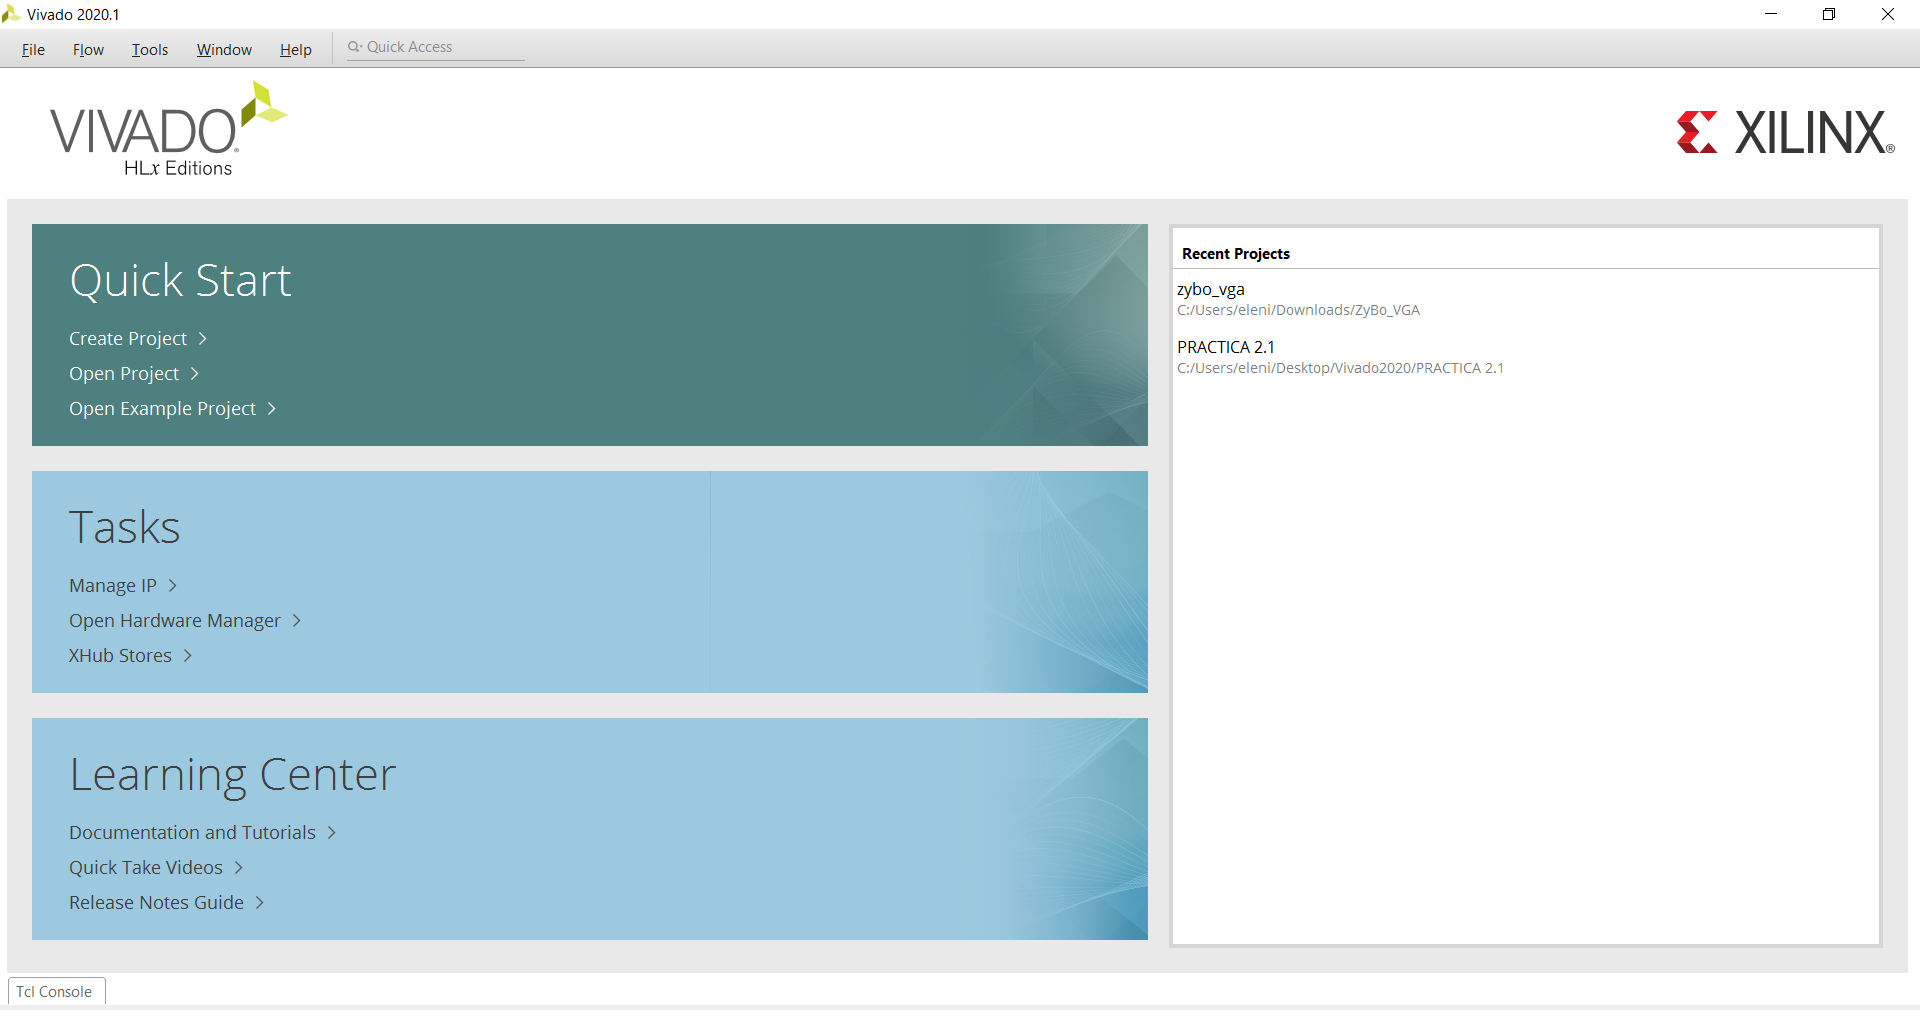
\includegraphics[width = 1\textwidth]{imagenes/Vivado1.png}
    \caption{Vivado IDE}\label{vivadoGUI}
\end{figure}

La sección \textbf{Quick Start} nos proporciona fácil acceso a la creación de un nuevo proyecto, abrir proyectos existentes o abrir proyectos 
de ejemplo ofrecidos por Xilinx. Además, en la sección \textbf{Recent Projects} se pueden abrir proyectos usados recientemente.

En la sección \textbf{Tasks} encontramos el acceso a \textbf{Manage IP} que nos permite crear una ubicación IP  para configurar y administrar 
IPs de forma remota. Se puede usar el catálogo de IP de Vivado para personalizar la IP. \textbf{Open Hardware Manager} nos ayuda a programar 
el diseño en el dispositivo. \textbf{Xilinx TCL Store} es un repositorio de código TCL. Da acceso a múltiples scripts para resolver problemas y 
mejorar la productividad.

La última sección es \textbf{Information Centre} donde se encuentra el acceso directo a la documentación, tutoriales y videos sobre lo que se 
puede hacer con esta herramienta.

Los componentes principales de la imagen \ref{vivado2} son:
\begin{enumerate}
    \item \textit{Menu Bar} \ref{menubar}
    \item \textit{Main Toolbar} \ref{maintoolbar}
    \item \textit{Flow Navigator} \ref{flownavigator}
    \item \textit{Layout Selector} \ref{Layoutselector}
    \item \textit{Data Windows Area} \ref{data}
    \item \textit{Workspace} \ref{workspace}
    \item \textit{Menu Command Search Field} \ref{mcsf}
    \item \textit{Project Status Bar} \ref{psb}
    \item \textit{Results Windows Area} \ref{status}
\end{enumerate}

\begin{figure}[H]
    \centering
    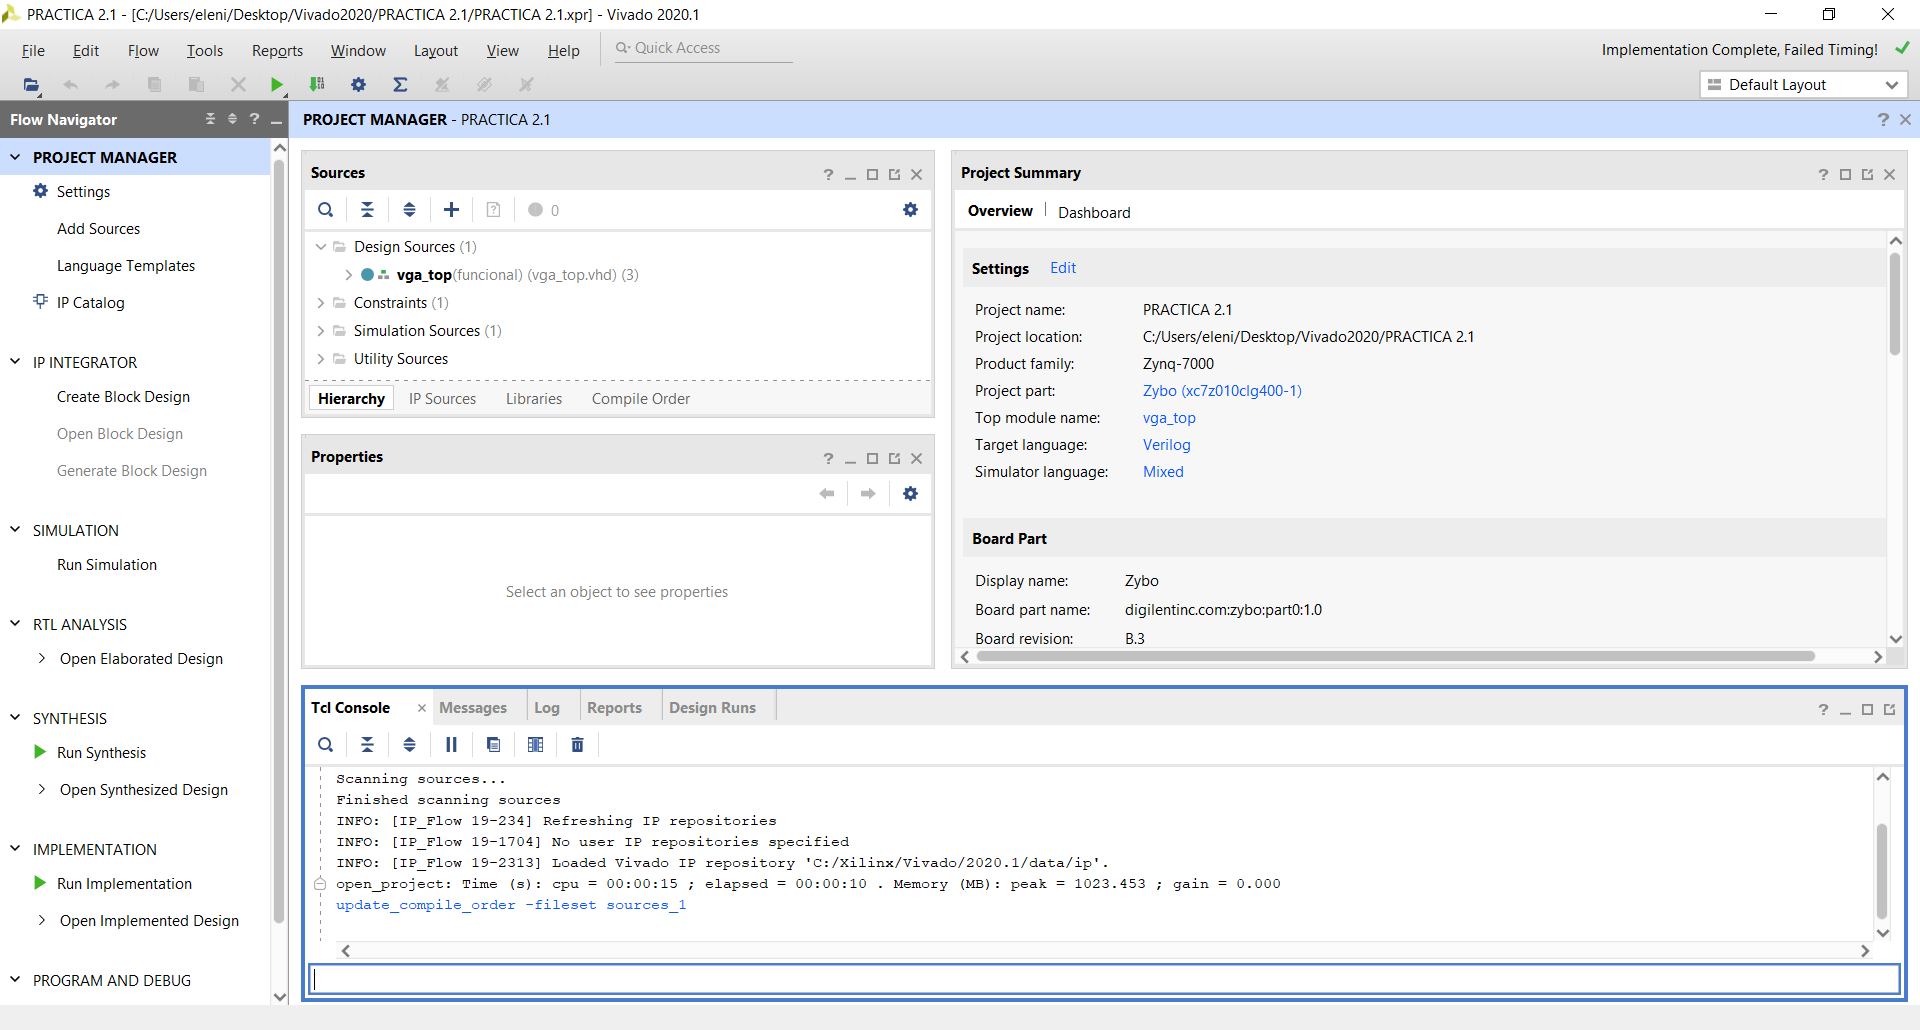
\includegraphics[width = 1\textwidth]{imagenes/vivado2.png}
    \caption{Entorno Principal Vivado IDE}\label{vivado2}
\end{figure}

\textit{Menu Bar} nos da acceso a los comandos de Vivado IDE. Normalmente, cuando se inicia un proyecto, no todos los comandos están 
disponibles, sino que algunos se muestran cuando el diseño está activo.

\begin{figure}[H]
    \centering
    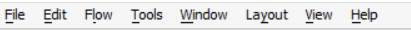
\includegraphics[width = 0.7\textwidth]{imagenes/menubar.png}
    \caption{\textit{Menu Bar}}\label{menubar}
\end{figure}

\textit{Menu Command Search Field} se encuentra a la derecha del anterior y permite localizar y ejecutar un comando de manera más rápida. La 
lista de comandos que aparecen en la búsqueda están basados en el contexto del proyecto del diseño actual.

\begin{figure}[H]
    \centering
    
\includegraphics[width = 0.5\textwidth]{imagenes/mcsf.png}
    \caption{\textit{Menu Command Search Field}}\label{mcsf}
\end{figure}

\textit{Main Toolbar} nos da acceso a los comandos más usados en Vivado IDE. Si se pone el cursor en alguno de estos comandos, Vivado 
ofrece más información acerca del mismo.

\begin{figure}[H]
    \centering
    
\includegraphics[width = 1\textwidth]{imagenes/maintoolbar.png}
    \caption{\textit{Main Toolbar}}\label{maintoolbar}
\end{figure}

\textit{Flow Navigator} permite acceder a comandos y herramientas que van desde abrir diseños a crear un archivo bitstream. Las 
diferentes secciones permiten hacer lo siguiente:
\begin{itemize}
    \item \textit{\textbf{Project Manager}}: Cambio de ajustes generales, añadir o crear archivos o abrir el Catálogo de IPs
    \item \textit{\textbf{IP Integrator}}: Crear, abrir o generar un bloque de diseño. 
    \item \textit{\textbf{Simulation}}: Cambio de ajustes de simulación o simular un diseño activo.
    \item \textit{\textbf{RTL Analysis}}: Abrir un diseño elaborado o generar un diseño de diagrama de circuitos RTL.
    \item \textit{\textbf{Synthesis}}: Cambio de ajustes de síntesis, sintetizar un diseño activo o abrir el diseño sintetizado.
    \item \textit{\textbf{Implementation}}: Cambio de ajuste de implementación, implementar un disñeo activo o abrir el diseño implementado.
    \item \textit{\textbf{Program and Debug}}: Cambio de ajustes del bitstream, generar un archivo bitstream o abrir una sesión hardware.
\end{itemize}

\begin{figure}[H]
    \centering
    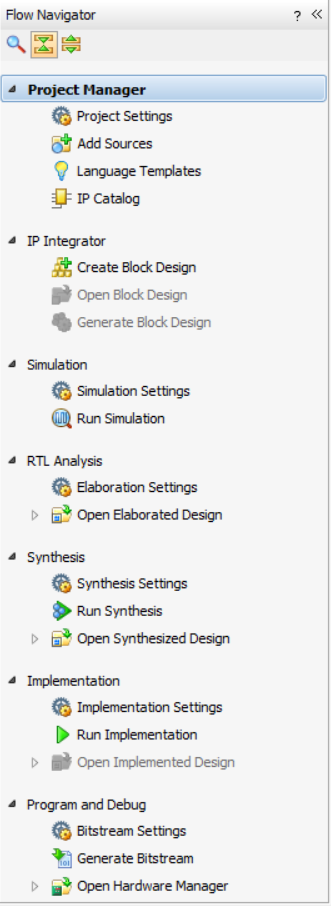
\includegraphics[width = 0.5\textwidth]{imagenes/flownavigator.png}
    \caption{\textit{Flow Navigator}}\label{flownavigator}
\end{figure}

\textit{Layout Selector} proporciona el diseño de ventanas predefinidas para facilitar el proceso de diseño. Entre las opciones tenemos:
\begin{itemize}
    \item \textit{\textbf{Default Layout}}: Analización del diseño con el mínimo número de ventanas
    \item \textit{\textbf{I/O Planning}}: Definición de restricciones de ubicación I/O y colocación de puertos.
    \item \textit{\textbf{Clock Planning}}: Planificación y colocación de los recursos del reloj del diseño.
    \item \textit{\textbf{Floorplanning}}: Gestionar particiones y tareas jerárquicas.
    \item \textit{\textbf{Timing Analysis}}: Ejecutar informes de tiempo y analizarlo.
\end{itemize} 

\begin{figure}[H]
    \centering
    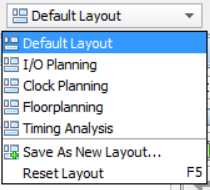
\includegraphics[width = 0.5\textwidth]{imagenes/Layoutselector.png}
    \caption{\textit{Layout Selector}}\label{Layoutselector}
\end{figure}

\textit{Project Status Bar} da información sobre el estado actual del diseño activo.

\begin{figure}[H]
    \centering
    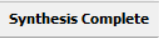
\includegraphics[width = 0.3\textwidth]{imagenes/psb.png}
    \caption{\textit{Project Status Bar}}\label{psb}
\end{figure}

\textit{Data Windows Area} muestra información sobre los archivos que forman el diseño.

\begin{figure}[H]
    \centering
    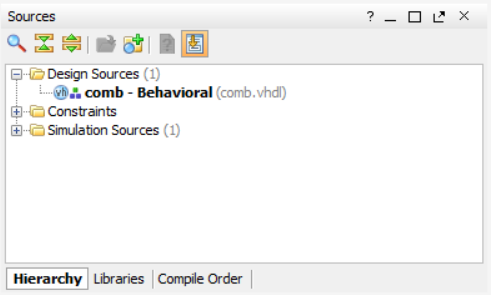
\includegraphics[width = 0.7\textwidth]{imagenes/datawa.png}
    \caption{\textit{Data Windows Area}}\label{data}
\end{figure}

\textit{Workspace} muestra ventanas como el editor de textos o el diseño del diagrama de circuitos, entre otros.

\begin{figure}[H]
    \centering
    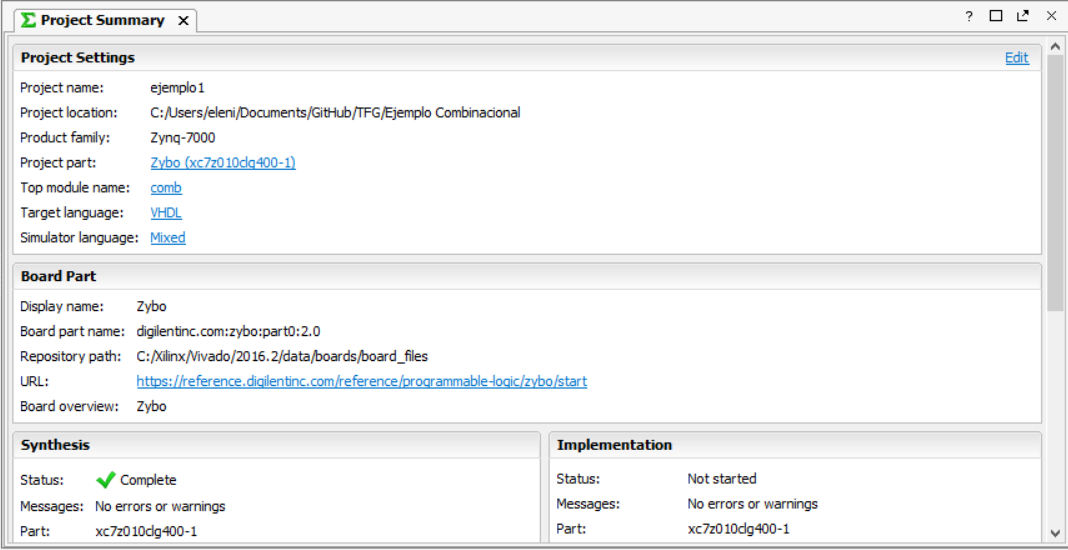
\includegraphics[width = 0.7\textwidth]{imagenes/workspace.png}
    \caption{\textit{Workspace}}\label{workspace}
\end{figure}

\textit{Results Windows Area} presenta los resultados de los comando ejecutados. Además se muestran distintas ventanas, como 
\textit{Tcl Console}, \textit{Messages}, \textit{Log}, \textit{Reports} y \textit{Design Runs}.

\begin{figure}[H]
    \centering
    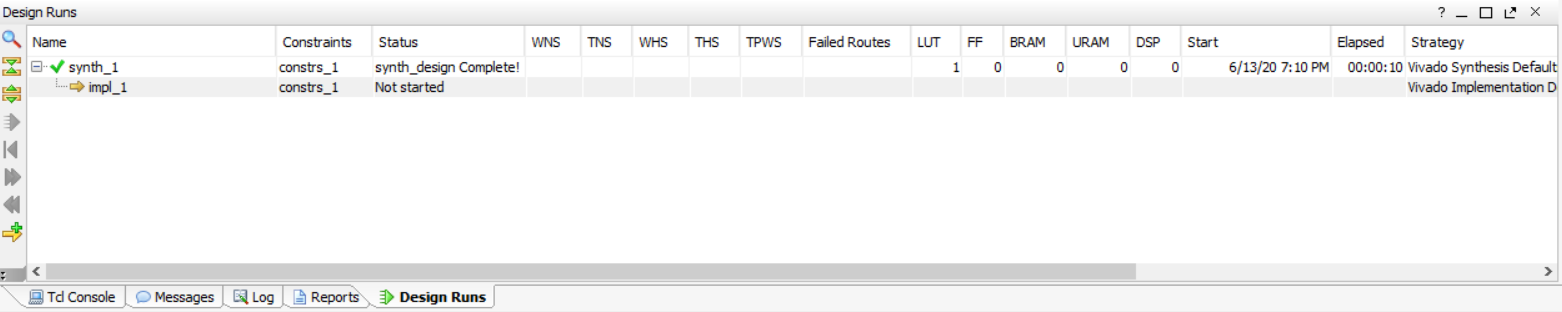
\includegraphics[width = 1\textwidth]{imagenes/statusbar.png}
    \caption{\textit{Results Windows Area}}\label{status}
\end{figure}

\section{Metodología}

\section{Desarrollo de módulos hardware específicos}

\section{Casos prácticos}
